\subsection{Cloud-Native}
\label{subsec:cna}

The definition of the cloud-native term is often mistakenly reduced to simply hosting applications in the cloud rather than on-premises \cite{gannon_2017}. In reality, cloud-native refers to a comprehensive software methodology for creating, deploying, and managing modern applications in dynamic computing environments \cite{davis_2019}. Cloud-native software is highly distributed, designed to operate in a constantly changing environment, and is inherently ephemeral.

To establish a scientifically sound foundation, this research adopts the definition provided by the Cloud Native Computing Foundation (CNCF), which serves as the definitive industry standard \cite{cncf_2026}. According to the CNCF, cloud-native technologies empower organizations to build and run scalable applications in public, private, and hybrid clouds. The foundational pillars of this architecture are microservices, containerization, automation, and immutable infrastructure as depicted in Figure \ref{fig:cncf-pillars}.

\begin{figure}[ht]
    \centering
    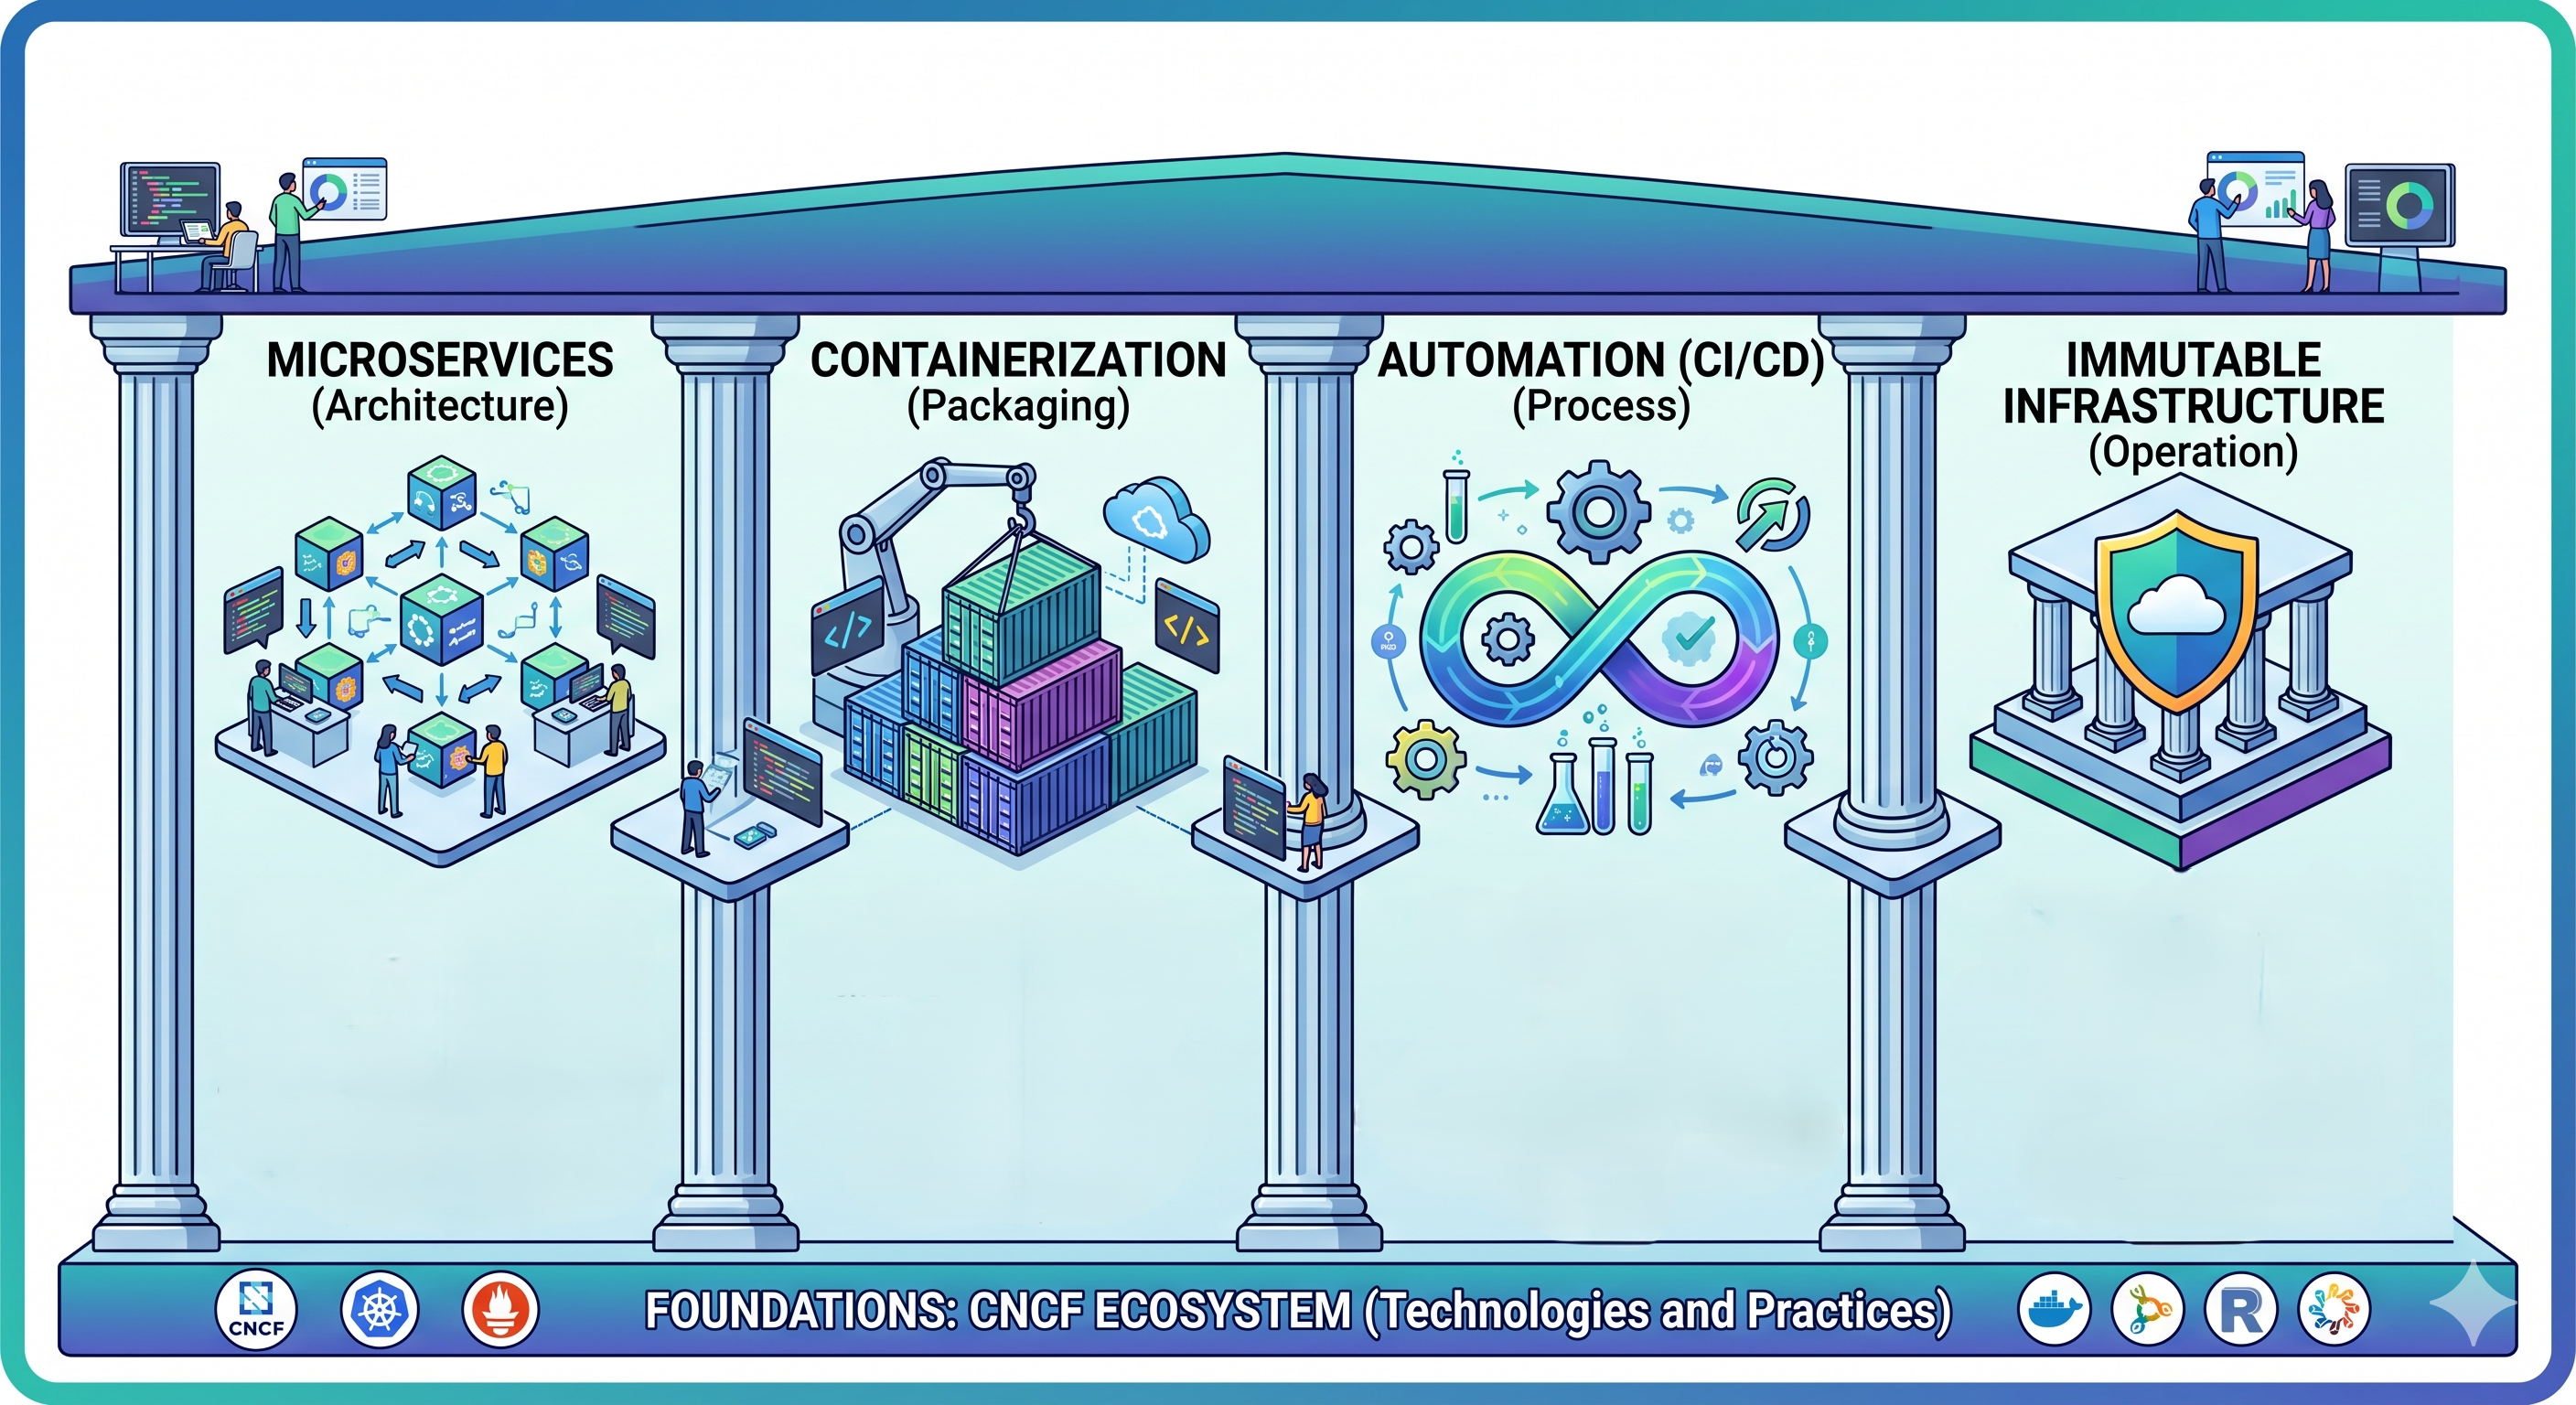
\includegraphics[width=1.0\linewidth]{images/cloud-computing/cncf-pillars.png}
    \caption{CNCF Pillars}
    \label{fig:cncf-pillars}
\end{figure}

Containers ensure that the application and its dependencies are packaged into a single, isolated unit of execution \cite{davis_2019}. Microservices decompose monolithic structures into small, independent processes communicating via lightweight mechanisms \cite{di_francesco_2019}. Meanwhile, declarative APIs and immutable infrastructure ensure that the system's state is automated and predictable, closely aligning with the Twelve-Factor App methodology \cite{twelve_factor_2017}. The concept of automation is directly related to the IaC section and, as will be explored in more depth in that topic, can be defined as the ability to execute tasks in a deterministic, sequential, and parameterizable manner, ensuring consistency across environments \cite{morris_2016}.

Together, these pillars enable loosely coupled systems that are resilient, manageable, and highly observable. However, this same highly distributed nature—where organizations no longer rely on centralized, monolithic systems—introduces an unprecedented level of complexity in analyzing infrastructure problems \cite{bhatia_2025}. Understanding this complexity is essential, as it forms the very baseline problem that the PANOPTES architecture is designed to monitor and diagnose.